\label{fram-intr}
As we have already said, we had to design a framework in such a way that our algorithms can share and exploit specific functionalities. In this context, it becomes useful to give a general view of the whole system by identifying and defining its abstraction layers, as shown in Figure~\ref{levels}. Let's briefly comment each of this levels and then focus on their specific features.
\begin{figure}[h]
  \begin{center}
    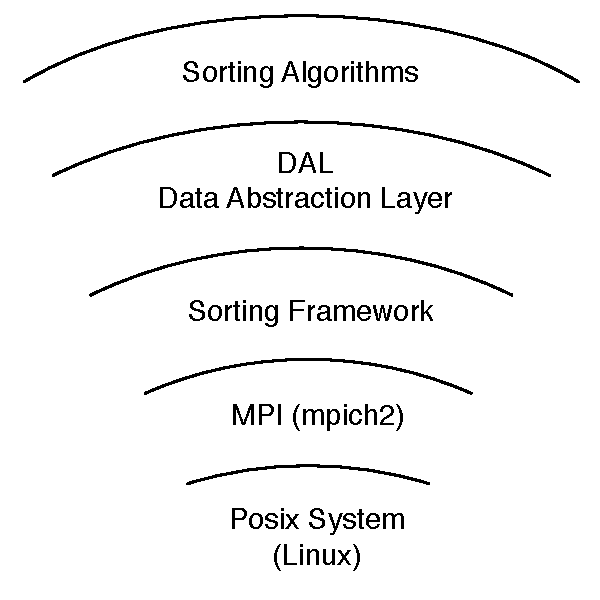
\includegraphics[scale=0.60]{levels}
  \end{center} 
  \caption{Abstract model}
  \label{levels}
\end{figure}
\begin{enumerate}
\item \textbf{Sorting Algorithms.} The logic of a parallel sorting algorithm is defined at this level. The programmer exploits the services provided by the Sorting Framework and works on primitives and data types provided by the DAL. As we will better explain later, we want to notice the fact that no visibility of MPI is provided at this level; for instance, processes of a parallel algorithm communicate with each other by means of the communication primitives provided by the DAL.  
\item \textbf{Sorting Framework.} At this level we implemented a set of functionalities that are common and essential to every sorting algorithm: the main ones are generation of data, loading data sets, storing results and taking and storing times.
\item \textbf{Data Abstraction Layer.} DAL is the fundamental layer of the system. It allows us to decouple the design of both the framework and parallel algorithms from the necessity of handling data sets that could not fit the primary memory. 
\item \textbf{MPI.} The DAL layer has been built on top of MPI, a well-known communication library between processes. Beyond the abstractions of communication, MPI is very useful for its capability of handling the deployment of the processes on a target architecture. There are some specific implementation of MPI, like \textit{mpich2}, that provide the user with a powerful deployment tool; in particular, we have interest in the possibility of specifying on which node a certain process must be allocated. By exploiting this feature we have been able to implement, for the same algorithm, different mappings of processes to nodes in order to study, for a given architecture, the communications impact on the performance. 
\item \textbf{Posix System (Linux).} Almost all the upper levels exploit Posix mechanisms, e.g. for gathering times, argument parsing, dynamic loading and the I/O functions to work with large files. This is quite important because Linux becomes the only platform on which is possible to run the application. 
\end{enumerate}
In some sense, we can say that starting from a tool for parallel programming like MPI, we designed a new tool, namely the run-time support of the Sorting Algorithm level, that addresses our needs for implementing parallel sorting algorithm for large data sets. 

In the following we are going to describe each of these levels starting from the top-most one, namely Sorting Algorithms. The emphasis will be obviously put on the first layers (Sorting Algorithms, Sorting Framework, DAL) which mainly represent the work we made in this project.

